\documentclass[10pt,utf8,presentation,notheorems,xcolor=dvipsnames,compress]{beamer}
\usepackage{doclad}
\usepackage{longtable}



\title[Приложение OptiTune]{
Приложение OptiTune 
}

\author[Касьяненко В.М.]{
  Касьяненко Вера Михайловна
}



\date{14 октября 2020}

\begin{document}

\begin{frame}
\titlepage
\end{frame}

\section<presentation>*{Содержание}

\begin{frame}
\frametitle{Содержание}
\vskip -0.75cm
\tableofcontents
\end{frame}

\section{Введение}
\begin{frame}[fragile,t]
\frametitle{Введение}
\begin{block}{}
В данном отчете будет представлена основная идея мобильного приложения OptiTune. Будет приведен интерфейс, описаны функции и основные пользователи приложения, а также будет проведена оценка рынка.
\end{block}
\end{frame}

\section{Описание будущего приложения}
\begin{frame}[fragile,t]
\subsection{Основная идея будущего приложения OptiTune}
\frametitle{Основная идея будущего приложения OptiTune}
\begin{block}{}
Мобильное приложение OptiTune предназначено для использования профессиональными стрелками, охотниками и военными. 
\end{block}
\begin{block}{}
С помощью приложения OptiTune пользователи смогут быстрее и качественнее подобрать необходимый тюнинг, улучшая там самым качество стрельбы.
\end{block}
\begin{block}{}
OptiTune позволит посмотреть характеристики и 3D-вариант тюнинга для гладкоствольного и нарезного оружия.
\end{block}
\end{frame}

\subsection{Основные функции приложения и интерфейс}
\begin{frame}
\frametitle{Основные функции приложения и интерфейс}
\vskip -0.35cm
  \begin{columns}[T]
    \begin{column}{.65\textwidth}
     \begin{block}{}
\begin{itemize}
\item подбор тюнинга на основе выбранного пользователем оружия
\item просмотр тюнинга в 3D-варианте отдельно и на оружии
\item просмотр и сравнение характеристик запчастей
\item добавление в избранное понравившегося тюнинга
\item написание и просмотр комментариев пользователями
\item оценивание тюнинга пользователями по различным критериям
\item помощь онлайн-консультанта
\end{itemize}
    \end{block}
    \end{column}
    \begin{column}{.25\textwidth}
    \begin{block}{}
	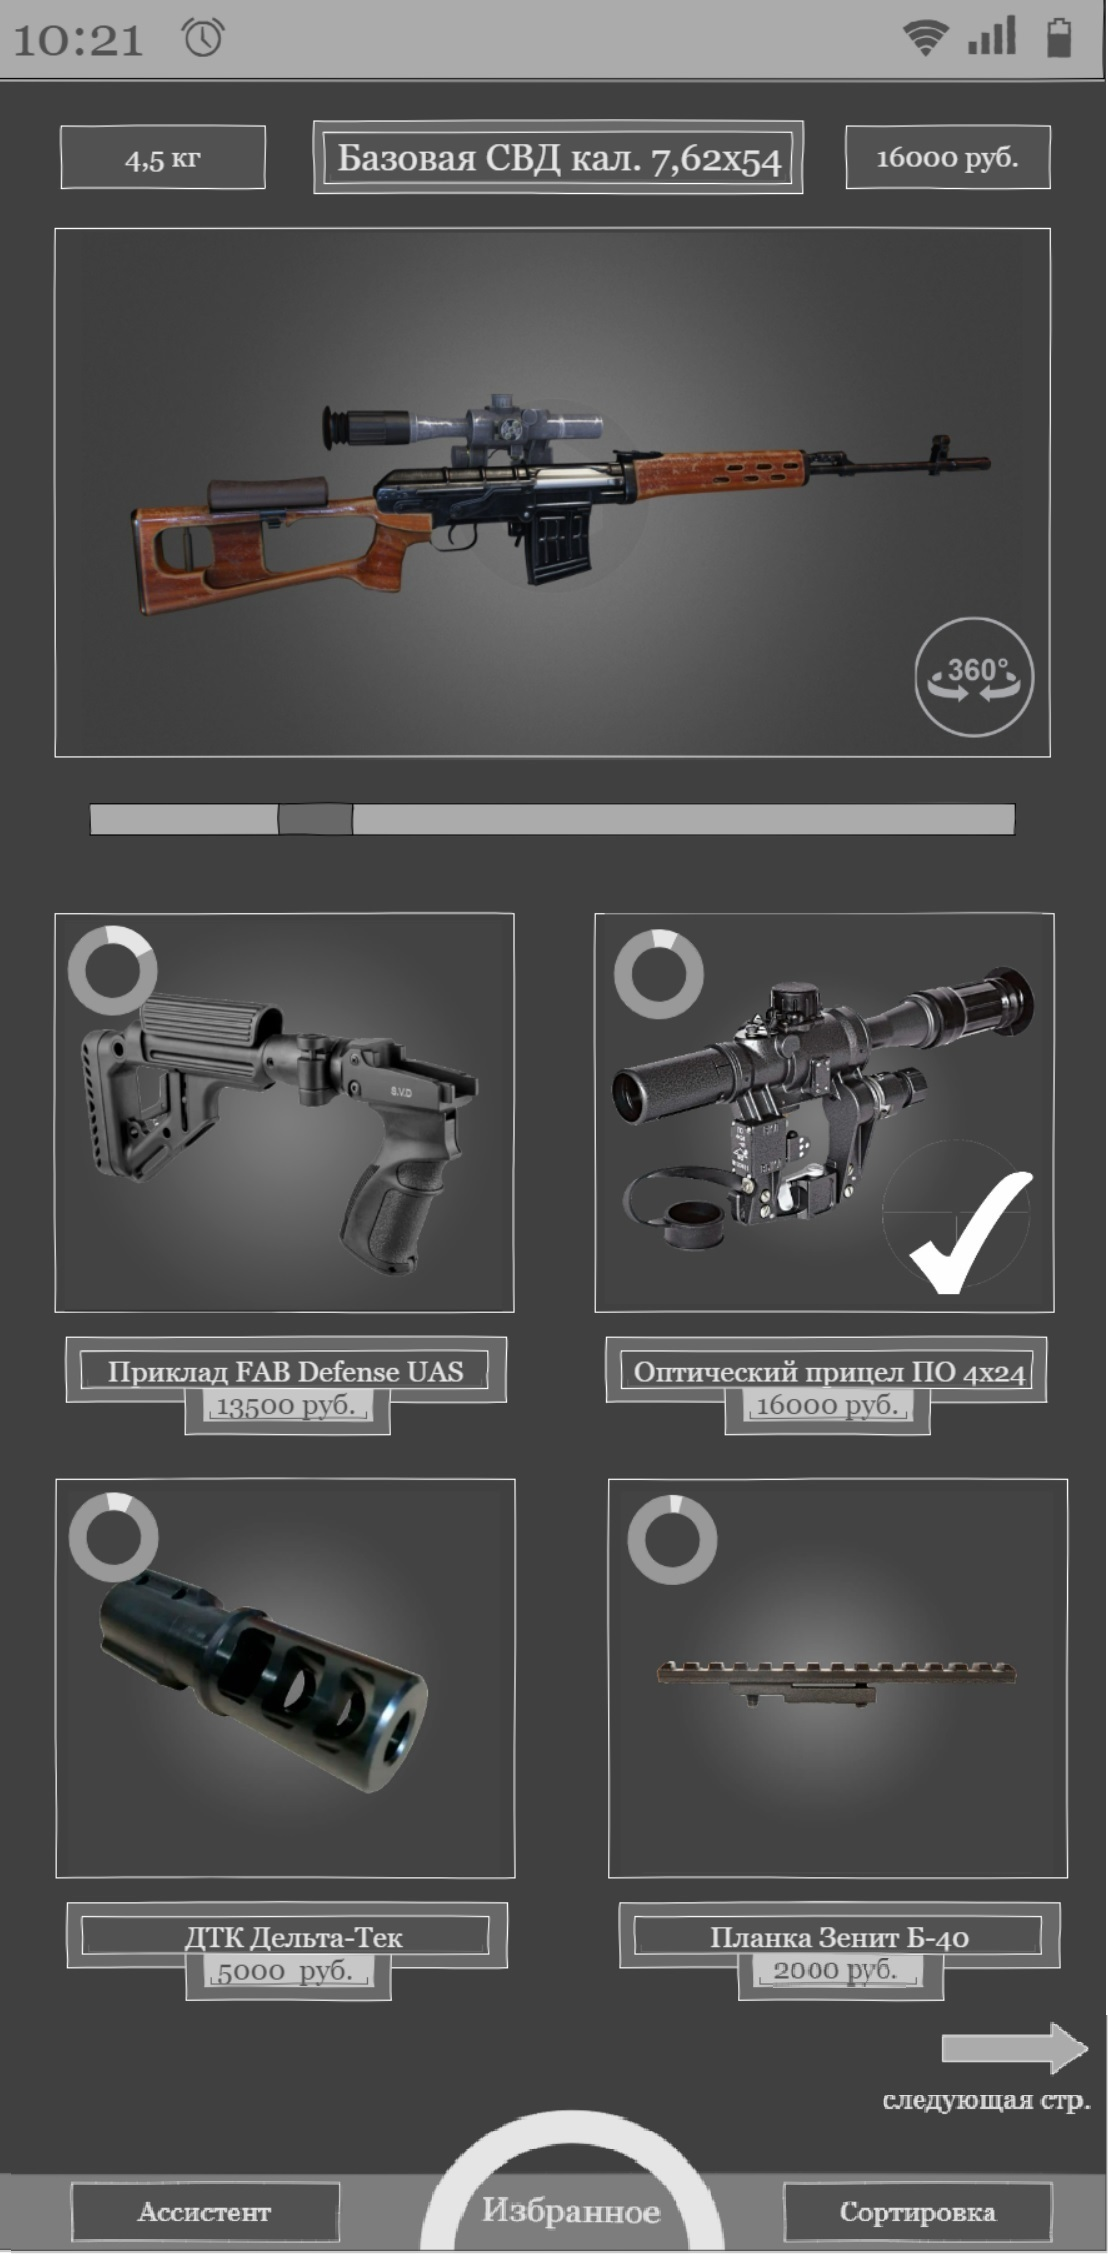
\includegraphics[scale=0.135]{pic}
    \end{block}
    \end{column}
  \end{columns}
\end{frame}

\subsection{Основные пользователи приложения и доступные им функции}
\begin{frame}
\frametitle{Основные пользователи приложения и доступные им функции}
\vskip -0.55cm
  \begin{columns}[T]
    \begin{column}{.65\textwidth}
     \begin{block}{Незарегистрированные пользователи}
\begin{itemize}
\item Подбор и просмотр тюнинга
\item Сравнение запчастей
\item Добавление в избранное
\item Просмотр комментариев и оценок пользователей
\end{itemize}
    \end{block}
    \vskip -0.15cm
     \begin{block}{Зарегистрированные пользователи}
\begin{itemize}
\item Подбор и просмотр тюнинга
\item Сравнение запчастей
\item Добавление в избранное
\item Просмотр и написание комментариев, а также оценивание запчастей
\item Помощь онлайн-консультанта
\end{itemize}
    \end{block}
    \end{column}
    \begin{column}{.25\textwidth}
         \begin{block}{Модератор}
\begin{itemize}
\item Просмотр и удаление комментариев
\end{itemize}
    \end{block}
    \vskip -0.175cm
         \begin{block}{Консультант}
\begin{itemize}
\item Помощь пользователям
\item Ответы на вопросы пользователей
\end{itemize}
    \end{block}
    \vskip -0.175cm
         \begin{block}{Менеджер}
\begin{itemize}
\item Обновление информации в приложении
\end{itemize}
    \end{block}
        \end{column}
  \end{columns}
\end{frame}

\section{Оценка рынка}
\subsection{Сравнение с аналогами}
\begin{frame}[fragile,t]
\frametitle{Сравнение с аналогами}
\vskip -0.15cm
\begin{table}[H]

\begin{center}
\begin{tabular}{|p{3,3cm}|c|c|c|c|}
\hline
 & OptiTune & Custom Guns & QUARTA & Guns Parts \\
\hline
Регистрация 

пользователей & Да & Нет & Да & Да\\
\hline
Поиск и сортировка запчастей & Да & Да & Да & Да\\
\hline
Просмотр 

характеристик & Да & Да & Да & Да\\
\hline
Сравнение 

характеристик & Да & Нет & Нет & Нет\\
\hline
3D-просмотр & Да & Нет & Нет & Нет\\
\hline
Добавление в 

избранное & Да & Нет & Да & Да\\
\hline
Комментирование пользователями & Да & Да & Да & Да \\
\hline
Онлайн-консультант & Да & Да & Да & Да\\
\hline
Покупка запчастей & Нет & Да & Да & Да\\
\hline
\end{tabular}
\end{center}
\end{table}
\end{frame}



\subsection{Обоснование необходимости создания приложения}
\begin{frame}[fragile,t]
\frametitle{Обоснование необходимости создания приложения}
\begin{block}{}
\begin{itemize}
\item Отсутствие конкуренции на рынке
\item Нет точных аналогов
\item Функции, которые смогут заинтересовать профессиональных стрелков
\item Удобство при подборе тюнинга
\end{itemize}
\end{block}
\end{frame}



\section{Заключение}

\begin{frame}[fragile,t]
\frametitle{Заключение}
\begin{block}{}
Был составлен отчет, в котором представлена идея приложения OptiTune, описаны основные функции и пользователи, а также приведен прототип интерфейса будущего приложения. Более того, был проведен анализ рынка, на основе которого были составлены некоторые выводы.
\end{block}
\end{frame}

\section{}

\begin{frame}

\frametitle{}
\centering
\begin{huge}
Спасибо за внимание!
\end{huge}
\end{frame}
\end{document}
